\documentclass[runningheads]{llncs}
\usepackage{amsmath}
\usepackage{amssymb}
\usepackage{graphicx}

\usepackage[usenames, dvipsnames]{color}
\usepackage{multirow}
\usepackage{subfig}
\usepackage{tabularx}
\newcolumntype{L}[1]{>{\raggedright\arraybackslash}p{#1}}
\newcolumntype{C}[1]{>{\centering\arraybackslash}p{#1}}
\newcolumntype{R}[1]{>{\raggedleft\arraybackslash}p{#1}}

\usepackage{listings}

\begin{document}

  \title{Predicting and Analyzing League of Legends Matches}
  \author{Benson Chen \and Kevin Lei}
  \institute{University of Pennsylvania}
  \maketitle
  
  \section{Introduction}  

	League of Legends is a multiplayer online battle arena (MOBA) game created by the video game publisher, Riot Games. Although there are many different game modes, the most common type is a 5v5 where players are separated into two teams of five. A players is known as a summoner and each summoner controls a champion which has a set of unique abilities and attributes. Before the start of the game, each team chooses their champions and other settings. The goal is for the teams to battle each other using their champions, using items and experience that are obtained in-game. The game’s currency is gold which can be obtained from killing enemy champions or killing third party characters (minions and jungle camps). There are also a variety of structures assigned to each team, one of them being the nexus. The game ends when one team is able to successfully destroy the other team’s nexus.

	LoL is on the forefront of the Esports scene along with other games such as Dota and Starcraft. Every year, Riot Games hosts an world championship tournament. In 2015, the LoL world championship was held in several locations, ranging from Berlin to Paris. In 2015, the average game had a concurrent viewership of 4.2 million unique viewers. To put that in perspective, the average episode of season 5 Game of Thrones has around 7-8 million viewers. The prize pool for the 2015 LoL world champions amounted to over 2 million USD. 
	
	In fact, LoL is so popular that some players stream themselves playing the game for a living. They do so through an online platform called Twitch, where a streamer can get up to 30-40 thousand viewers at a time. In peak hours, the viewership of Twitch rivals that of popular cable networks like MTV, Comedy Central, MSNBC and CNN. Through ad revenue and donations from viewers, these gamers support themselves by simply playing the LoL game.

	For these reasons, we want to look at an aspect of League of Legends, analyzing what factors contribute to a team winning.

	\section{Goals}
	
	This project has two main goals:
	\begin{enumerate}
		\item
		Create a model that predicts the probability of win given match statistics.
		
		\item
		Find out what variables contribute most to winning a game, so that we can create strategies that will give better chances of winning the game.		
	\end{enumerate}
	
	For the first goal, it may not make much sense to use the match information to predict the probability of winning since the match will have already happened by then. However, there are other uses. One use is that this model can be a good proxy for predicting the probability of winning when the game is still happening. League of Legends is a heavily broadcasted Esport and having a measure of how the game is progressing is an important metric. For instance, by using logistic regression, we get a probability of how likely a team is likely to win. While the game is being played, knowing this metric can better provide viewers with an estimate of how much of an advantage one team has over the other team at that point in time.
	
	For the second goal, we really want to look at what variables most indicative of a winning match-up. Using this information, we can construct strategies that can give teams a sense of what they should strive to do during the game to get an advantage.
	
	\section{Data Collection}

	The first step in our project was collecting the data from Riot’s League of Legends API. We used two of the endpoints: (1) match-v2.2; (2) matchlist-v2.2. The first endpoint, match-v2.2, returns information related to a given match. Specifically, it takes a matchId (unique identifier for each match) as a parameter and returns a data structure containing statistics relating to the participants, teams, and events within the game. The second endpoint, matchlist-v2.2, returns match information for a given summoner (someone who plays LoL). The endpoint takes a summonerId (unique identifier for each summoner) and returns a list of matches that the summoner has played. We narrowed down our data set to ranked 5v5 games played in 2015 season.

To accomplish this task, we wrote a Java program which uses these two endpoints to acquire a list of summoners and then subsequently a list of matches.

To acquire a list of summoners, we used two methods: getMatches and getSummoners. The first method, getMatches, takes a summonerId and calls the matchlist-v2.2 endpoint to obtain all of the matches that the summoner has played. This list then gets written to a file. The second method, getSummoners, takes matchId and uses the match-v2.2 endpoint to obtain the list of summonerIds which had participated in that given match. Using these two methods in conjunction allowed us to randomly obtain a large number of matches. Firstly, we picked a random seed summonerId. We passed this into getMatches and chose a random match to obtain new summoners. We constructed two queues to hold a list of potential summonerIds and matchIds and continuously called the two methods in a loop, using getMatches to add more matchIds to the match queue and using getSummoners to add more summonerIds to the summoner queue. If we imagine a graph of summonerIds where the vertices are matchIds and edges connect matches with the same participants, we traversed the graph using a Depth First Search (DFS) to obtain our list of matches.

After obtaining our list of matches, we used a different method, populateMatches, which took in a matchId and called the match-v2.2 endpoint to obtain features for each match. The method parsed the JSON output to obtain information about the champions used in each match, gold received by each team during a given time frame, wards and items bought and used, and other features relevant to a team’s success. We have outlined a more specific description of the features in the Data Overview section below.

	\section{Data Cleaning}
	
	After obtaining our raw data from our Java program, our next step was to clean the data. Our first concern was that Riot’s API did not always return well-formed JSON. This resulted in some of the features containing null values or empty strings. Since we could always use our program to obtain more matches, we simply removed any matches with these malformed features. This left us with a cleaned dataset of 3,000 matches.

We also removed any features from our dataset that were not useful. For example, we had indicator variables for each championId. In particular, championId of 420 corresponded to Illaoi, a champion released about a month ago for the 2016 season. Since we had only collected data for matches in the 2015 season, we never saw this champion used and subsequently removed its corresponding indicator variable.
	
	\section{Data Overview}
	
	In this section, we summarize our data and give descriptions for our features.
	
	\subsection{Sample Size}
	
	We use a sample of 3,000 random matches of LoL games.
	
	\subsection{Response Variable}
	
	Our response variable is categorical 1-0 variable that is 1 if \textcolor{blue}{team 1} wins, and 0 if \textcolor{red}{team 2} wins.
	
	\subsection{Champions}
	
	The first and obvious feature that we included was the champions themselves. Excluding the newest champion Illaoi, for which we do not have data, there are 127 total champions. To simplify our task, we approached this feature in the following manner:

	\begin{center}
		\begin{tabular}{ |l|l| }
			\hline
			Champion is on \textcolor{blue}{team 1} & Assigned a value of 1 \\ \hline
			Champion is on \textcolor{red}{team 2} & Assigned a value of -1 \\ \hline
			Champion is not in current game & Assigned a value of 0 \\ \hline
		\end{tabular}
	\end{center}
	
	We could have used separate indicator variables for champions being on teams 1 or 2, but we wanted to limit the size of our feature space in order to guarantee that our methods ran fast enough.
	
	We see from the following table the summary statistics of the frequency of champions played (on either team):
	
	\begin{center}
		\begin{tabular}{ |L{2cm}|L{2cm}|L{2cm}|L{2cm}|L{2cm}|L{2cm}| }
			\hline
			Minimum & 1st Qt. & Median & Mean & 3rd Qt. & Maximum \\ \hline
			14.0 & 83.5 & 159.0 & 236.2 & 350.5 & 1166.0 \\ \hline
		\end{tabular}
	\end{center}
	
	We see that there is a wide range of frequencies for how often a champion is played--this is unsurprising. There are some champions that are played very frequently, while there are others that are rarely played. According to the above, the average champion was played in 236.2 or $7.83\%$ of the games.
	
	\begin{figure}
		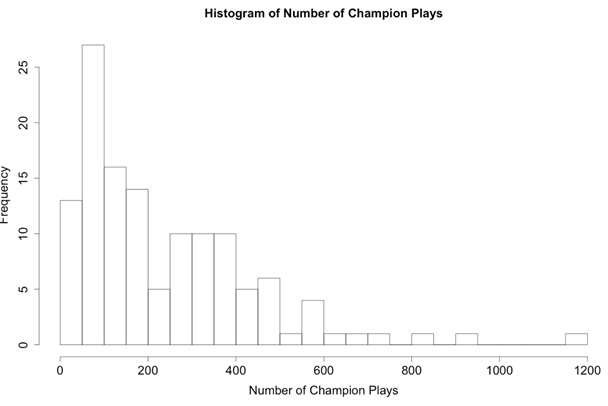
\includegraphics[width=\textwidth]{images/hist_champions.png}
		\caption{Histogram of the number of times a champion is played}
	\end{figure}
	
	From the histogram, we see that there is a pretty significant right skew. Again, this is not extremely surprising as there are a few champions that are played very frequently, while other champions are rarely being played.

	In fact, the top three most popular champions were Thresh (1166 games), Janna (914 games) and Lee Sin (824 games). It is unsurprising that the top two are Thresh and Janna because they are found in the support roles, and there is usually less variety in the champions that you can pick for the support roles.
	
	\begin{figure}
		\centering
		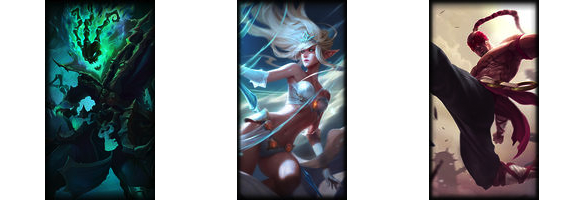
\includegraphics[width=0.45\textwidth]{images/top_3.png}
		\caption{From left to right: Thresh (38.9\%), Janna (30.5\%) and Lee Sin (27.5\%)}
		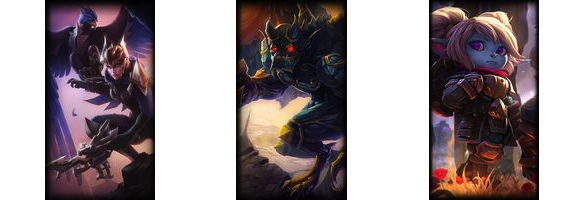
\includegraphics[width=0.45\textwidth]{images/bot_3.png}
		\caption{From left to right: Quinn (0.05\%), Galio (0.06\%) and Poppy (0.06\%)}
	\end{figure}
	
	The bottom three least popular champions were Quinn (14 games), Galio (17 games), and Poppy (17 games). This is also unsurprising as these champions are typically considered much weaker than most other champions.

	\subsection{Minions and Jungle Camps}
	
	In a LoL game, you want to earn gold to buy items that make you stronger. There are several ways of earning gold including killing the other team, killing minions and jungle camps. If you have more gold than your opponent, you will be at a significant advantage, because your spells and attacks will deal significantly more damage.

	\begin{figure}
		\centering
		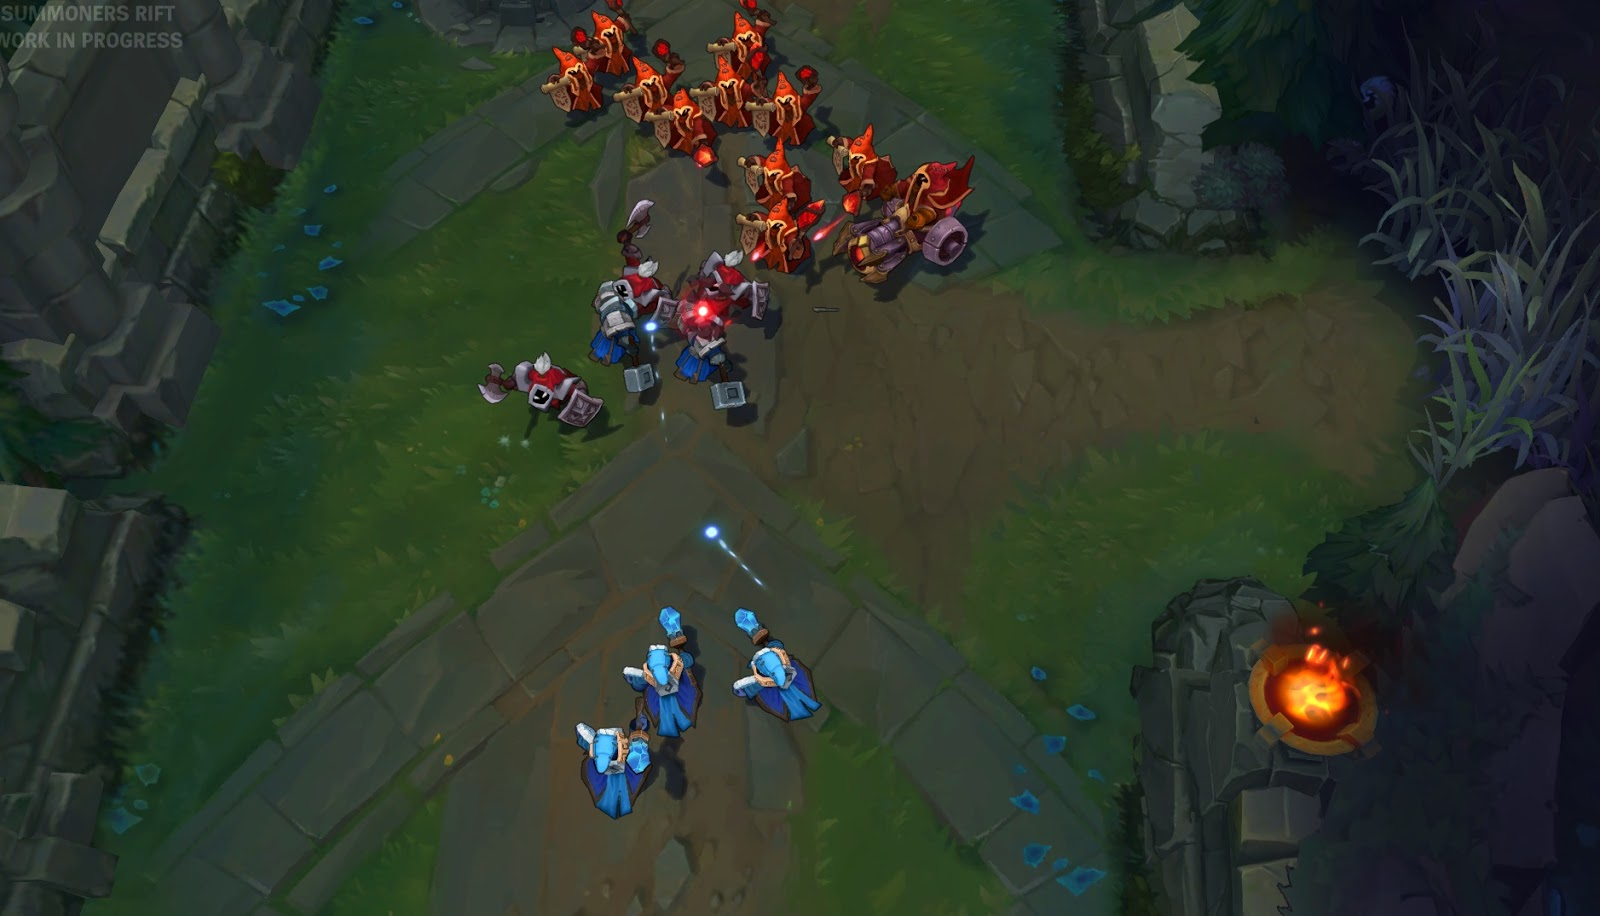
\includegraphics[width=0.5\textwidth]{images/minions.jpg}
		\caption{An example of a minion camp}
	\end{figure}

	The most steady stream of income is from killing minions and jungle camps, because you never know when and if you are able to kill the enemy champions. Therefore, if you are able to kill a lot more minions than your opponent, you will naturally have more gold, which you can use to purchase items that increase your damage. 

	\begin{figure}
		\centering
		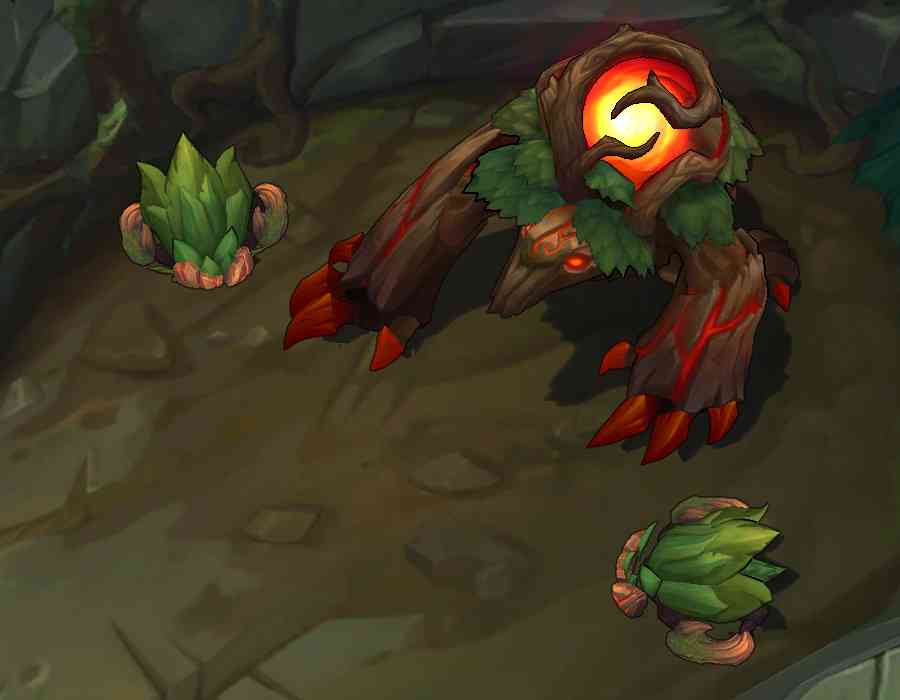
\includegraphics[width=0.5\textwidth]{images/jungle.jpg}
		\caption{An example of a jungle camp}
	\end{figure}

	There are five roles in LoL, Top, Mid, ADC, Jungler and Support. There are some differences with how each role obtains gold as listed below. 
	
	\begin{center}
		\begin{tabular}{ | L{2cm} | L{3cm} | }
			\hline
			Top & Kill Minions \\ \hline
			Mid & Kill Minions \\ \hline
			ADC & Kill Minions \\ \hline
			Jungler & Kill Jungle Camps \\ \hline
			Support & - \\ \hline						
		\end{tabular}
	\end{center}
	
	The support role usually does not have a steady stream of income, as the support player does not usually kill any minions or jungle camps for gold. Instead, they rely on their team getting kills of the other team’s champions to get gold. 

	The jungler is different from the other roles in that the jungler kills jungle camps for gold instead of regular minions. 

	For minions, we use a statistic called minions per minute, or MPM, which as the name suggests, describes how many minions a champion has killed per minute. Because only three roles really kill minions, we look at the difference in MPM in the Top, Mid and ADC roles. While the support and junglers do kill some minions, they usually kill a small number, and so it does not make much sense to include features for these two roles.

	Additionally, we delve further and look at the differences in MPM between the two teams from 0-10 minutes and 10-20 minutes. We make this distinction, because the early game is most indicative of how people are doing. If a team wins, it’s obvious that their final minion count will be higher, but it is not obvious whether or not their initial minion kills will be higher. Perhaps they are giving up minion kills early in the game to secure other objectives.

	Because the only statistics we can find on jungle camps is the total number of jungle camps killed, we also include the difference in number of total jungle camps killed as a variable.

	Therefore, the 7 variables we include for minion/jungle camps kills are succinctly summarized in the following table:
	
	\begin{center}
		\begin{tabular}{ | L{3cm} | L{5cm} | }
			\hline
			\multirow{3}{*}{0 - 10 minutes} & Difference in MPM for Top \\
			& Difference in MPM for Mid \\
			& Difference in MPM for ADC \\ \hline
			\multirow{3}{*}{10 - 20 minutes} & Difference in MPM for Top \\
			& Difference in MPM for Mid \\
			& Difference in MPM for ADC \\ \hline
		\end{tabular}
	\end{center}
	
	\subsection{Wards}
	Wards are important, because they give vision of the opponent’s team. With wards, you can  better strategize during the game to exploit your opponent’s positioning. Similarly, if your opponent places a lot of wards on the map, they can see how your team is being positioned.

	Wards can be bought from the shop, or placed using certain items. Because wards cost money to buy, only a few roles, namely the jungle and support roles buy wards. This is because other roles would rather invest in damage items so that they can more easily kill their opponents. Therefore, we mainly concentrate on the difference of warding patterns between the jungle and support roles of the two teams.

	\begin{figure}
		\centering
		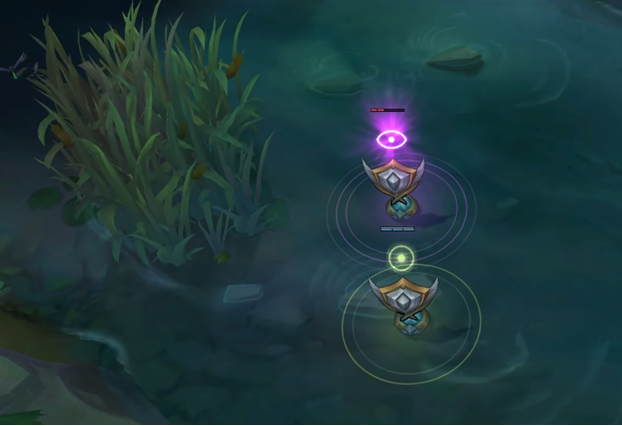
\includegraphics[width=0.5\textwidth]{images/wards.png}
		\caption{Stealth Ward (bottom) and Vision Ward (top)}
	\end{figure}
	
	All variables are considered in the context of the difference between the two teams. For instance, the difference in number of wards bought by the two teams would be:
	
	\begin{center}
		(wards bought by team 1) - (wards bought by team 2)
	\end{center}

	A positive difference would mean that team 1 is doing better, and a negative difference would indicate the exact opposite.

	There are two different types of wards that one can buy from the shop, sight and vision wards; however, because we feel that the total number is more important than knowing the specific distribution, we use the total number of wards bought.

	Another important variable to consider is the number of wards killed. Just as they can be placed, wards can also be killed by the other team. This is extremely important, because by destroying wards, you are eliminating the enemy’s vision of you. As mentioned earlier, vision is an extremely important part of the game, because it allows you to make more informed strategic movements during the game. Therefore, by destroying wards, it is expected that your opponents will make worse decisions, increasing the chance that you will win.
	
	\begin{center}
		\begin{tabular}{ | C{3cm} | L{7cm} | }
			\hline
			\multirow{3}{*}{Jungle} & Difference in number of total wards bought \\
			& Difference in number of wards placed \\
			& Difference in number of wards killed \\ \hline
			\multirow{3}{*}{Support} & Difference in number of total wards bought \\
			& Difference in number of wards placed \\
			& Difference in number of wards killed \\ \hline
		\end{tabular}
	\end{center}
	
	We see from the pairwise scatter plots (see Appendix) that there is no clear correlation between any of the wards variables. This is surprising, as you would expect that if the support on team 1 has bought a lot more wards than the support on the the other team, then they would have placed more wards as well. However, this could simply be because of the noise in the data.
	
	\subsection{First Blood}
	
	In LoL, ''first blood'' is the term used for the first kill of the game. In order to reward the champion that gets the first blood, that champion is given extra gold. Not only does the first blood give a physical advantage to the team that gets it, it also gives them a psychological advantage. This is because the team that had their champion killed first usually feels psychological stress of knowing that they are behind the other team. Therefore, we felt that the first blood variable might be predictive and important for strategic purposes.

	As a feature, the first blood variable is a simply binary variable that is 1 if team 1 got the first blood, and 0 if team 2 got the first blood.
	
	\subsection{Dragon and Baron}
	
	Besides killing minions, there are also two objectives, the dragon and the baron. Killing these two objectives can give your team a significant buff that greatly increases your chances of winning.

	\textbf{Dragon}. The dragon is available to be killed right at the start of the game. Killing the dragon disables the dragon, and no team can kill it again for another 6 minutes. Killing the dragon grants the killing team a permanent buff that includes things like greater damage, and more movement speed.

	\begin{figure}
		\centering
		
\includegraphics[width=0.4\textwidth]{images/dragon.png}
		\caption{Dragon}
	\end{figure}		

	\textbf{Baron Nashor}. The Baron Nashor, or Baron for brevity, spawns on the map at 20 minutes. Killing the Baron disables the Baron, and no team can kill it again for another 7 minutes. Killing the Baron grants the killing team a temporary buff that greatly increases the pushing strength of the team. This allows the team that get the buff to greatly speed up the pace of the game, and push for the win. 

	\begin{figure}
		\centering
		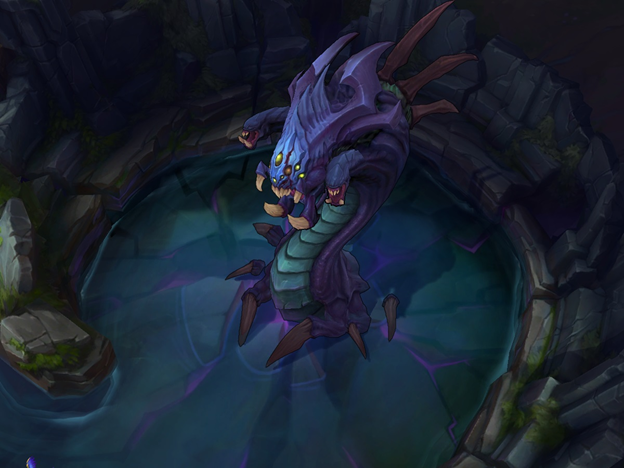
\includegraphics[width=0.4\textwidth]{images/baron.png}
		\caption{Baron Nashor}
	\end{figure}	

	In general, the Baron is much harder objective to take down compared to the dragon, and offers a much greater reward for taking it down. In our analysis, we consider the number of barons and dragons taken down by each team. Unlike the other variables, we do not use the difference in the number of dragons/barons slain, because the actual number matters. For instance, the more dragons you kill, the stronger the buffs are. 

	\begin{figure}[!htb]
		\centering
		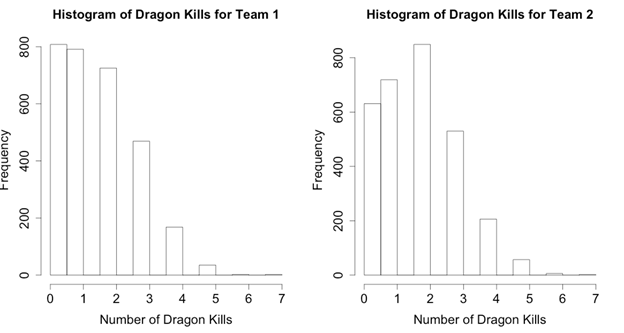
\includegraphics[width=\textwidth]{images/hist_dragon.png}
		\caption{Histogram of Dragon Kills}
	\end{figure}	

	\begin{figure}[!htb]
		\centering
		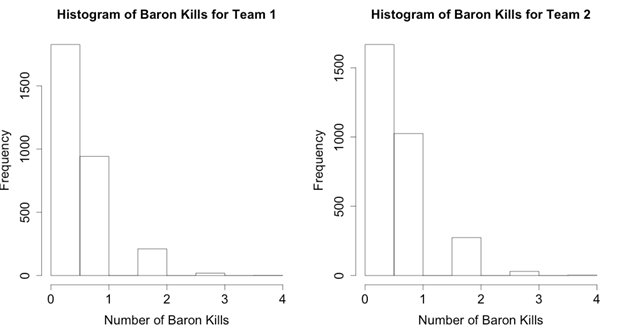
\includegraphics[width=\textwidth]{images/hist_baron.png}
		\caption{Histogram of Baron Nashor Kills}
	\end{figure}
	
	Therefore, in this category, we have a total of 4 variables, the number of barons and dragons taken by team 1 and 2.
		
	First, we notice that the distributions for team 1 and team 2 are similar. This is to be expected, as the teams that win should be randomly distributed. Second, we see that usually, a much higher number of dragons are killed. This is in-line with the fact that the dragon is much easier to kill, and does not give as big of an advantage. In fact, most games go through without a single baron kill.
	
	\section{Feature Selection}
	
	Because one of our main goals is interpretation, to find what strategic moves a team should utilize, we first want to use logistic regression to model the data. To do that, we use LASSO to do feature selection, because we have around 145 features from our cleaned dataset.
	
	\begin{figure}[!htb]
		\centering
		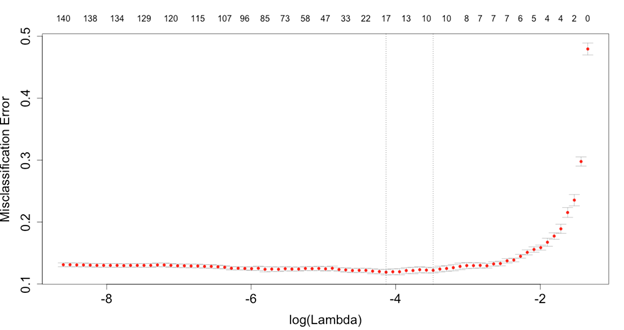
\includegraphics[width=\textwidth]{images/lasso.png}
		\caption{MCE of LASSO using 10-fold CV}
	\end{figure}
	
	The above graph plots the misclassification error against the $\log(\lambda)$ values in a 10-fold cross validation setting. We see that as $\log(\lambda)$ decreases, the misclassification error asymptotically levels off. Because it seems like we have found a reasonable minimum, we do not have to try other values of lambda.

	The right dashed line indicates a $\log(\lambda)$ value that is 1SE above the minimum. I chose to use a lambda value slightly to left of the 1SE in order to get a few more variables. Using a $\log(\lambda)$ value of -3.8, we got a reasonable number of variables, twelve, so we ended up using these features.

	The twelve selected important variables are as follows, with a description as a reminder of what they are, and why they are important:
	
	\begin{center}
		\begin{tabular}{ | l | L{7cm} | }
			\hline
			Top MPM 0-10 & This is the difference in  minions per minute score for the Top role, from 0 to 10 minutes. \\ \hline
			Top MPM 10-20 & This is the difference in minions per minute score for the Top role, from 10 to 20 minutes. \\ \hline
			Mid MPM 10-20 & This is the difference in minions per minute score for the Mid role, from 10 to 20 minutes. \\ \hline
			ADC MPM 0-10 & This is the difference in minions per minute score for the ADC role, from 0 to 10 minutes. \\ \hline
			ADC MPM 10-20 & This is the difference in minions per minute score for the ADC role, from 10 to 20 minutes. \\ \hline
			Difference in Jungle Camps Kills & This is the difference in the total number of jungle camps killed. \\ \hline
			Difference in Number of Wards Placed by Support & This is the difference in number of wards placed by the support. Recall that wards are important because they give you vision of the enemy team, and allow you to better make decisions during the game. \\ \hline
			First Blood & This indicates the team that got the first kill during the game. \\ \hline
			Number of Dragon Kills by Team 1 & This is the number of dragons killed by team 1. Recall that dragons give a permanent buff to the team that killed it, but this buff is much weaker than the Baron Buff. \\ \hline
			Number of Dragon Kills by Team 2 & This is the number of dragons killed by team 2. Recall that dragons give a permanent buff to the team that killed it, but this buff is much weaker than the Baron Buff. \\ \hline
			Number of Baron Kills by Team 1 & This is the number of barons killed by team 1. Recall that barons give a very powerful temporary buff \\ \hline
			Number of Baron Kills by Team 2 & This is the number of barons killed by team 2. Recall that barons give a very powerful temporary buff. \\ \hline
		\end{tabular}
	\end{center}	
	
	\section{Logistic Regression}
	
	We then use logistic regression to create a model to both predict win rate, as well as to investigate the important strategical factors of gameplay.
	
	To do so, we split our data into 2 sections, a train set and a test set. Because we have 3,000 data points, we decided to use 2,000 of it as training data, and the other 1,000 as testing data.

	The output of our logistic regression is as follows

	\begin{figure}[!htb]
		\centering
		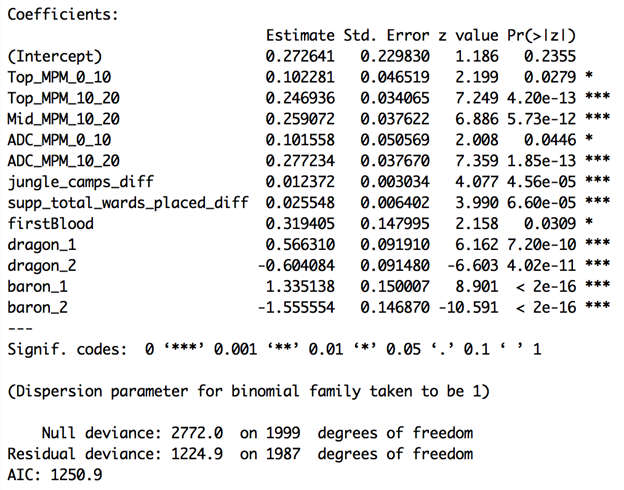
\includegraphics[width=\textwidth]{images/lr_summary.png}
		\caption{Summary of Logistic Regression coefficients}
	\end{figure}
	
	\begin{align*}
	\log \left( \frac{Pr[win]}{1 - Pr[win]} \right) =&\; 0.27 + 0.10 * (\text{Top MPM 0-10}) + 0.25 * (\text{Top MPM 10-20}) \\
	& + 0.26 * (\text{Mid MPM 10-20}) + 0.10 * (\text{ADC MPM 0-10}) \\
	& + 0.28 * (\text{ADC MPM 10-20}) + 0.012 * (\text{Jungle Camp}) \\
	& + 0.026 * (\text{Wards Placed by Supports}) + 0.32 * (\text{First Blood}) \\
	& + 0.57 * (\text{Dragons Team 1}) - 0.60 * (\text{Dragons Team 2}) \\
	& + 1.34 * (\text{Barons Team 1}) - 1.56 * (\text{Barons Team 2})
	\end{align*}
	
	
	
	We immediately see that the MPM (minions per minute) variable is extremely important. This comes as no surprise, because the more MPM you achieve, the more gold you earn, and the better items you can buy. Items can then make you deal more damage, and allowing you to achieve an even higher MPM or even kill the enemy’s champions, creating a positive feedback loop. In fact, for the 10-20 minutes range, an increase in 1 more minion killed per minute correlates to an average increase of 0.26 in the log odds ratio.

	What is interesting is while the MPM values for ten to twenty minutes were all significant, only the MPM values for top and ADC are significant for the zero to ten minutes range. This is probably because if the MPM value for zero to ten minutes range is highly correlated with the MPM in the next ten minutes. Therefore, the model is probably not benefiting much from having these extra variables, so we remove the MPM for top and ADC in the zero to ten minutes range variables. We do a likelihood ratio test on the two nested models, and get a p value of less than 5\%. Therefore, it’s reasonable to say that there is not a significant difference between the two models, and we go with the simpler model.
	
	\begin{figure}[!htb]
		\centering
		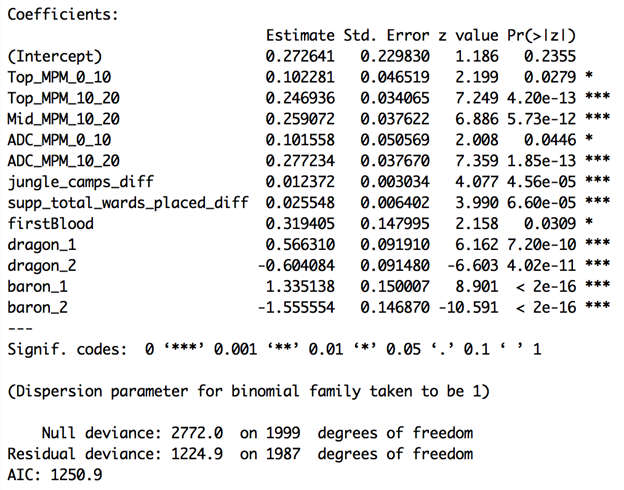
\includegraphics[width=\textwidth]{images/lr_simple.png}
		\caption{Simpler Model for Logistic Regression}
	\end{figure}
	
	\begin{align*}
		\log \left( \frac{Pr[win]}{1 - Pr[win]} \right) =&\; 0.27 + 0.27 * (\text{Top MPM 10-20}) + 0.26 * (\text{Mid MPM 10-20}) \\
		& + 0.30 * (\text{ADC MPM 10-20}) + 0.012 * (\text{Jungle Camp}) \\
		& + 0.025 (\text{Wards Placed by Supports}) + 0.37 * (\text{First Blood}) \\
		& + 0.58 * (\text{Dragons Team 1}) - 0.62 * (\text{Dragons Team 2}) \\
		& + 1.32 * (\text{Barons Team 1}) - 1.57 * (\text{Barons Team 2})
	\end{align*}
	
	Next we see that the number of jungle camps killed is also important. This is essentially a proxy for how well one jungler is doing compared to the other jungler. An increase in 1 total jungle camp killed correlates to an average increase in 0.0122 of the log odds ratio. This coefficient is much smaller than the MPM one, because that is a rate per minute, whereas this statistic is the total number killed.

	We see that most of the wards features were not selected by LASSO, except for the difference in number of wards placed. For each additional ward that the support places more than the opponent, there is a correlation of an increase of 0.0254 in the log odds ratio of winning. It is unsurprising that the more wards the support places, the greater the chance of winning, because wards are such an important strategic aspect of the game. However, it is surprising that this was the only ward variable that was selected through LASSO.

	We also see that there is a positive correlation in getting the first blood and winning. More specifically, being on the team that secures first blood correlates to an average increase of 0.370 in the log odds ratio of winning. This is expected, because getting the first blood gives the team a substantial gold lead early game, which they can use to kill their opponents over and over again. Additionally, on a psychological level, getting the first blood gives the team a morale boost, and when players feel like they are winning, they are probably likely to perform better.

	On the matter of the objectives of dragons and barons, we once again see results that we would expect: positive coefficients for dragons and barons that your team kills and negative coefficients for dragons and barons that your opponent’s team slays. This is because both objectives give a significant boost to the killing team’s strengths. It is interesting to note that an additional baron or dragon that your opponent gets creates a greater difference in the log odds ratio of winning than dragons or barons that your own team secures. However, this difference may not be statistically significant.

	What we do not see as important features are the champions themselves. This is unsurprising because Riot Gaming constantly balances champions so that they are not too strong or too weak. Therefore, we would expect that no one champion would consistently outperform other champions, all else held equal.

	Next, we look at how well our model predicts the win rate. As a reminder, out the 3,000 data points, we used 2,000 of them for the training data, and 1,000 data points are left as testing data.

	We obtain the following confusion matrix using a threshold of $50\%$, weighing both wins and losses equally. This has a misclassification error of $12.7\%$.


	\begin{center}
		\begin{tabular}{ | L{3cm} | C{2cm} | C{2cm} | }
			\hline
			& Predicted Loss & Predicted Win \\ \hline
			Actual Loss & 479 & 66 \\ \hline
			Actual Win & 61 & 394 \\ \hline
		\end{tabular}
	\end{center}
	
	Additionally, we see that our model achieves an AUC of 94.12\%.
	
	\begin{figure}[!htb]
		\centering
		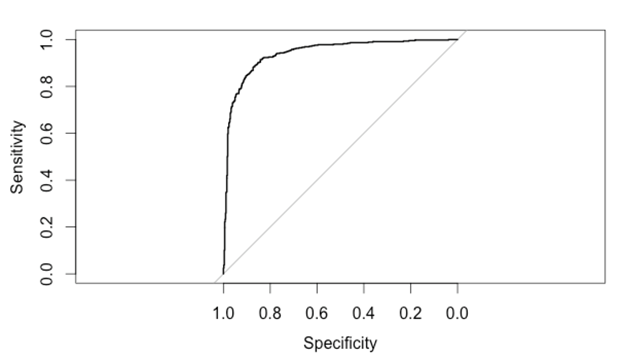
\includegraphics[width=0.7\textwidth]{images/lr_roc.png}
		\caption{ROC for Logistic Regression}
	\end{figure}
	
	It is unsurprising that our model is able to do so well. This is because certain factors of the match statistics is very predictive. If a team has secured many Baron objective kills, their team is much more likely to win, because the Baron gives such a huge buff to the team. Therefore, it is unsurprising that a simple model like LR can predict very accurately the outcome of the game. 

	To reiterate our original goals, we want a predictive model as a proxy to judge the outcome of the game while the match is happening. That is, we want to be able to use this model, say after the 20 minutes mark, to judge how much more one team is winning compared to the other. And the LR model is one method for which we can use to do this. Another, which we explore next, is using random forests.
	
	\section{Random Forest}
	
	We then approached our problem using a non-parametric method, creating a Random Forests 
model. More specifically, we used the training set created for the Logistic Regression model and limited the number of variables per tree to 10. 

	We measured the importance of each variable by looking at each variable’s impact on the Gini coefficient (see Figure 15). We found that the number of dragon and baron kills were the most significant in predicting a win which conforms with our prior knowledge that these types of kills provide significant advantages to the team.
	
	\begin{figure}[!htb]
		\centering
		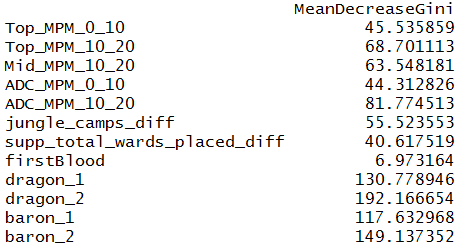
\includegraphics[width=0.5\textwidth]{images/rf_importance.png}
		\caption{Importance of Variables in Random Forest}
	\end{figure}
	
	We also see that firstBlood is the least important variable, confirming the results form the Logistic Regression model where firstBlood had a small coefficient. This is because getting the first kill is not a huge advantage and can sometimes make a team overconfident and risk-seeking.
	
	\begin{figure}[!htb]
		\centering
		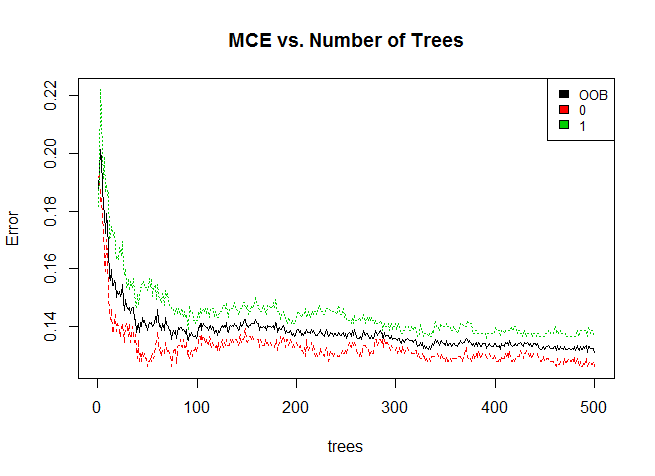
\includegraphics[width=\textwidth]{images/rf_mce.png}
		\caption{Classification error when using a different number of trees}
	\end{figure}
	
	Using the Out-Of-Bag error, we also looked at how Missed Classification Error varied with the number of trees. We saw that the at about 100 trees, adding additional trees had a small effect on lowering the MCE.
	
	\begin{center}
		\begin{tabular}{ | L{3cm} | C{2cm} | C{2cm} | }
			\hline
			& Predicted Loss & Predicted Win \\ \hline
			Actual Loss & 923 & 133 \\ \hline
			Actual Win & 129 & 815 \\ \hline
		\end{tabular}
	\end{center}	
	
	From our confusion matrix, we saw that when weighting both wins and losses equally, we had a missed classification error of 13.1\%, comparable to the Logistic Regression model.
	
	\begin{figure}[!htb]
		\centering
		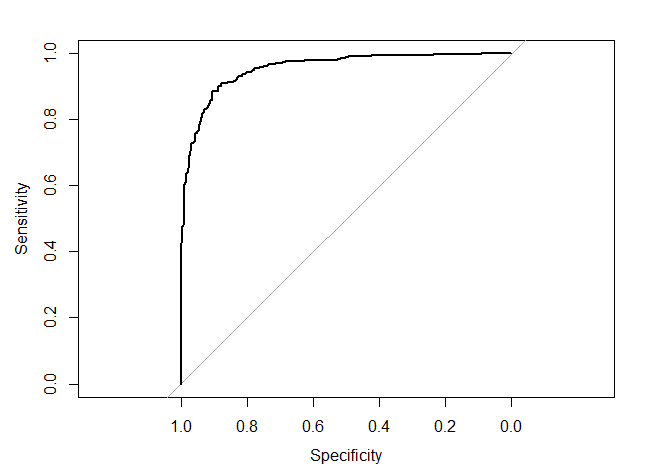
\includegraphics[width=0.7\textwidth]{images/rf_roc.png}
		\caption{ROC for Random Forest}
	\end{figure}
		
	The Random Forest model also achieves an AUC of 0.9551 which is slightly better than the Logistic Regression model. As stated before and with the same rationale, this model performs well. Using a nonparametric model that achieves similar results shows that our analysis and results are robust and does not rely heavily on certain assumptions.
	
	\section{Conclusion}
	
	In our analysis, we looked at two different models, logistic regression with feature selection and random forests. The logistic regression model not only offers us a predictive model, but also interpretation of the variables. It tells us how the response variable (likelihood of winning) is changed when the explanatory variables are changed.

	For logistic regression, we first did feature selection using LASSO. The main features that should be highlighted are the MPM for each of the three roles, Top, Mid and ADC, wards placed by the support, the team that got the first blood, as well as dragon and Baron objective kills.

	From a strategic standpoint, there are several important takeaways.
	
	\begin{enumerate}
		\item
		Being able to kill as many minions is very important. This is a test of the skill of the player, and to improve, players should work on their ability to kill as many minions as they can. No matter which of the three roles, Top, Mid, or ADC, this skill is very important.
		
		\item
		For supports, placing more wards is very important. This creates more vision for your team, and allows your team to make more informed decisions in-game.
		
		\item
		Being able to get first blood is important, but it is okay if your team isn’t the one to first kill an enemy champion. More important than the gold boost is probably the morale boost that the team gets from getting first blood.
		
		\item
		Dragon and Baron objective kills are very important. It is important to have tight control over these objectives, because they confer such a huge advantage to the team that kills these objectives.
	\end{enumerate}
	
	In terms of prediction, we see that our LR model did very well, achieving an AUC of 94.12\%. However, we proceeded to use random forest to see if we can do even better.

	While LR is a parametric model, random forests are completely non-parametric. This is good in several respects, because there are many non-linear relationships that exists in the data that can be captured by the random forests.

	Our RF model performed similarly with an AUC of 95.51\% and a MCE of 13.1\% The marginal improvement in performance is probably too small to be attributed to any assumptions in LR. This does tell us that our results are robust and that our analysis is consistent across two very different types of statistical models.
	
	\section{Limitations}
	
	There are many variables that we did not consider that are also important. For instance, each player can choose a set of runes and masteries, which give combat statistics to their champions. Additionally, the item purchases that each player chooses can also heavily affect his or her performance. However, there are simply too many combinations of items and therefore would not be feasible for this project.

	Additionally, a game of LoL is extremely dynamic, and we simply captured a few static variables, such as number of wards placed, or number of wards killed. There could be many confounding variables that lead to high numbers for number of jungle camps killed. 

	We also assumed that we knew which player chose which role. The Riot API gave its best guess as to which role it thought the player was, but roles are only loosely defined in the game. Therefore, there could be some inaccuracies in the data that we simply cannot account for. 

	It maybe more useful to limit our matches to a particular patch (update to the game), rather than the season (all the updates in a given year). By doing so, we probably would have seen some champions having significant contribution to a team’s victory. This is because during certain patches, some champions might be too overpowered, only to be fixed in a later patch.

	Furthermore, one of the most important things that we did not consider were the bans in a game. Before each player selects his or her champion, each team can decide to ban a certain number of champions, so that they cannot be played in that game.

	Nevertheless, despite the limitations and inaccuracies that may exist, we believe that we have constructed a model that adequately served our main two goals. One is to construct a model that can be used as a proxy to predict likelihood of winning as a matching is ongoing. The second is to find out what variables are the most impactful in order to determine what strategies will lead to the most victories.
	
	\section{Works Cited}

	\begin{enumerate}
		\item[]
		\url{http://www.lolesports.com/en\_US/all-star/articles/worlds-2015-viewership}
		
		\item[]
		\url{https://en.wikipedia.org/wiki/Game\_of\_Thrones}
		
		\item[]
		\url{http://loldevelopers.de.vu/}
		
		\item[]
		\url{https://developer.riotgames.com/api/}
		
		\item[]
		\url{http://www.nytimes.com/2014/08/26/technology/amazon-nears-a-deal-for-twitch.html}
	\end{enumerate}
	
	\section{Appendix}
	R code and Java program can be found at: \url{https://github.com/Kevin-Lei/stat471\_final\_proj}
		
	\begin{figure}
		\centering
		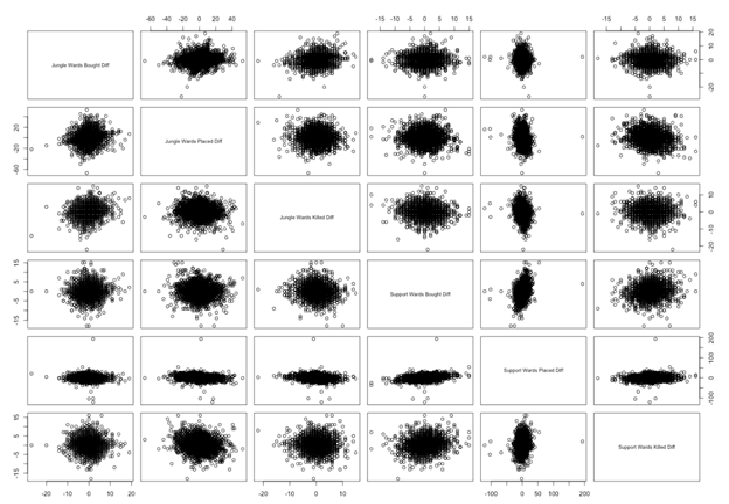
\includegraphics[width=1.0\textwidth]{images/pairwise_scatter.png}
		\caption{Pairwise scatter plots of selected variables}
	\end{figure}
	
%  \begin{figure}
%  \includegraphics[width=\textwidth]{protocol.png}
%  \caption{Overview of our verifiable computation protocol}
%  \end{figure}
  
\end{document}